\section{Durchführung}
\label{sec:Durchführung}
\subsection{Konzept der Messung}
\label{sec:Durchführung1}

Ohne äußeres Magnetfeld sind die Energieniveaus eines Elektrons in Bezug auf
ihren Spin entartet.
Beim Anlegen eines Magnetfeldes $\vec{B}$ spaltet sich das Niveau in Abhängigkeit
von dem Spin des Elektrons auf.
\begin{figure}
  \centering
  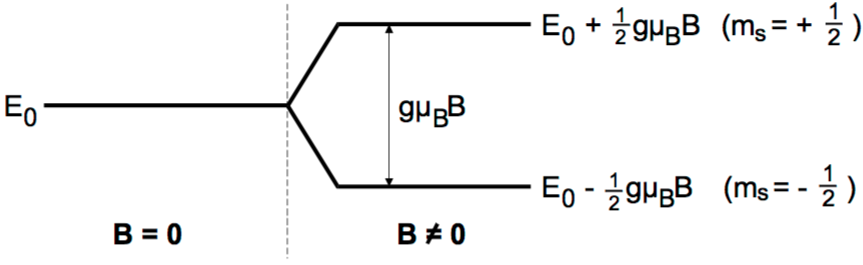
\includegraphics[width=0.6\textwidth]{graphics/energieaufspaltung.png}
  \caption{Schematische Aufspaltung eines Energieniveaus bei Anwesenheit von Magnetfeldern.\cite{skript}}
  \label{fig:energieaufspaltung}
\end{figure}
Die Energiedifferenz zweier Elektronen, die sich durch ihren Spin unterscheiden,
ist wie in Abbildung \ref{fig:energieaufspaltung} skizziert
\begin{equation}
  \mathup\Delta E = g\mu_B B.
\end{equation}
Diese Energiedifferenz wird messbar gemacht, indem eine Probe in ein homogenes
Magnetfeld einer konstanten Stärke eingelassen wird. Zusätzlich wird eine Spule,
die zum Betrieb bei hohen Frequenzen geeignet ist, um die Probe gewickelt und an
eine Brückenschaltung angeschlossen. Diese Brückenschaltung dient dem Messen der
Impendanz (komplexer Widerstand) der HF-Spule. Beim Anregen der Probe mit
hochfrequenten Magnetfelder wird bei einer bestimmten Frequent der in Abbildung
\ref{fig:energieaufspaltung} gezeigte Übergang angeregt, der sich in einer Änderung
der Proben-Magnetisierung äußert.
Diese Resonanz kann durch empfindliche Messgeräte durch auftretende Brückenströme
gefunden werden.

\subsection{Portrait der Messinstrumente}
Die HF-Spule wird in eine Brückenschaltung eingebaut und über einen präzisen Hochfrequenz-
Generator mit Wechselstrom gespeist. Durch die Stellelemente $R$ und $C$ wird die
Brückenschaltung so eingestellt, dass ohne das homogene Magnetfeld die Brückenspannung
verschwindet.

Da für die Messung eine hochpräzise Einstellung erforderlich ist,
wird die Spannung am Brückenausgang um Größenordnungen verstärkt und Störspannungen
unterdrückt. Dies geschieht durch einen Superheterodyn-Verstärker, dessen Aufbau
in Abbildung \ref{fig:superhomo} schemenhaft gezeigt wird.
\begin{figure}
  \centering
  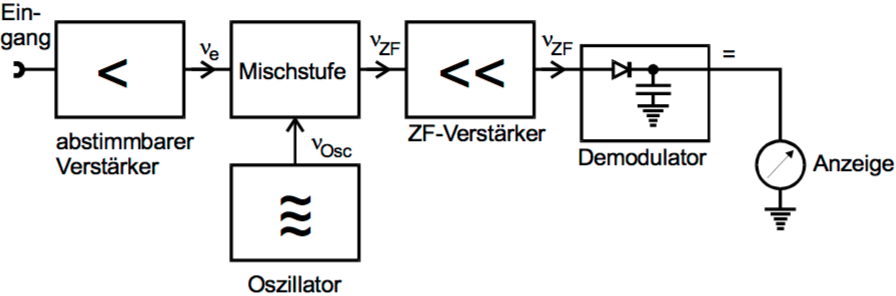
\includegraphics[width=0.6\textwidth]{graphics/superhomo.png}
  \caption{Skizzierter Aufbau eines Superheterodyn-Verstärkers. \cite{skript}}
  \label{fig:energieaufspaltung}
\end{figure}
Nachdem ein Vorverstärker das Signal geringfügig verstärkt und bei der Frequenz
$f_\text{Eingang}$ filtert, überlagert eine Mischstufe dieses vorgefilterte Signal
mit einem Signal geringerer Frequenz $f_\text{Osz}\approx f_\text{Eingang}$. Durch diese
Überlagerung treten Schwebungen auf, die das Abstimmen der Frequenzen
$f_\text{Eingang}$, $f_\text{Osz}$ erleichtern.
Die Schwebung mit der Frequenz $f_\text{Schwebung}=f_\text{ZF}=f_\text{Eingang}-f_\text{Osz}$
wird durch den anschließenden ZF-Verstärker wesentlich verstärkt, sodass ein Demodulator
ein gleichgerichtetes Signal als brauchbare Messgröße ausgeben kann. Der ZF-Verstärker
verstärkt dabei nur Frequenzen $f_\text{Schwebung}$ und ist damit ein wirksamer Filter
gegen Störfrequenzen $f\neq f_\text{Eingang}$ am Eingang des Superheterodyn-Verstärkers.

\subsection{Messvorgehen}
Die Feldspulen werden in Richtung des Erdmagnetfeldes aufgestellt. Durch Wiederholung
der Messung bei beiden Feldorientierungen, parallel und antiparallel zum Magnetfeld,
kann der Betrag des Erdmagnetfeldes bestimmt werden.

Nachdem eine Probenspule in das Brückengehäuse eingelassen wurde, wird die Oszillatorfrequenz
$f_\text{Osz}$ eingestellt. Für diese Frequenz muss $f_\text{Osz}=f_\text{ZF}+f_\text{Eingang}$
bei gegebenem $f_\text{Osz}$ gelten. Beim Anlegen einer hochfrequenten Spannung an
die Brücke wird eine Spannung am Ausgang des Superheterodyn-Verstärkers messbar.
Durch Einstellen des Vorverstärkers wird diese Spannung maximiert\footnote{Ggf. muss der
ZF-Verstärker herabgeregelt werden.}. Die Einstellung des Vorverstärkers wird über
den Versuch hinweg nicht variiert.
Anschließend wird mit den Stellelementen $R$ und $C$ dieselbe Spannung bei voller
ZF-Verstärkung minimiert; auch die $C$-Stellelemente werden nicht mehr wesentlich verändert,
könnten aber zwecks der Optimierung der Resonanzkurve angepasst werden.
Das $R$-Stellelement wird soweit verstimmt, dass eine Spannung von $\SI{150}{\milli\volt}$
bis $\SI{700}{\milli\volt}$ gemessen wird. Diese Verstimmung ermöglicht den Erhalt
einer Resonanzkurve in Gestalt von Abbildung \ref{fig:res_signal}. Wird keine Resonanzkurve
dieser, aber ähnlicher Form gefunden, muss das $R$-Stellelement weiter verstimmt werden.
\begin{figure}
  \centering
  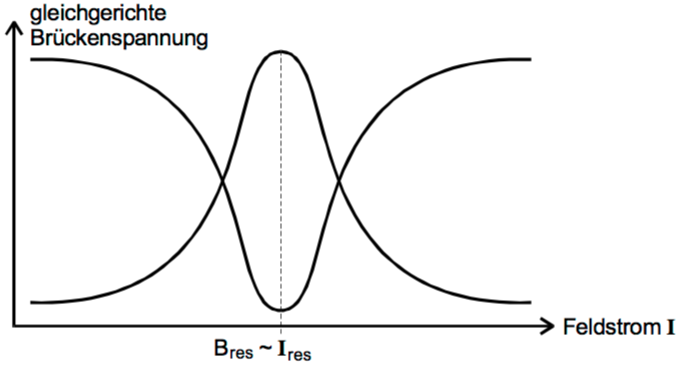
\includegraphics[width=0.6\textwidth]{graphics/res_signal.png}
  \caption{Gesuchte Resonanzkurve: Spannung $U$ am Ausgang des Verstärkers aufgetragen
  gegen die Feldstromstärke $I_\text{Feld}$. \cite{skript}}
  \label{fig:res_signal}
\end{figure}

Die Spulen werden mit Gleichstrom linear steigender Stärke versorgt. Hierzu steuert
ein Niederspannung-Rampengenerator einen Leistungsverstärker an, sodass mit $B\propto I\propto t$
zeitaufgelöst die Magnetfeldstärke variiert. Ein XY-Plotter, an dessen X-Eingang
die Feldstromstärke und an dessen Y-Eingang der Superheterodyn-Verstärker angeschlossen sind,
zeichnet einen Verlauf nach Abbildung \ref{fig:res_signal}, sofern das Spektrum
der Magnetfeldstärke geeignet ist. Mit der Eichung der X-Achse über ein gewöhnliches
Amperemeter kann die Resonanzfeldstärke mithilfe von
\begin{equation}
    B(I)= \frac{8}{\sqrt{125}}\mu_0\frac{n}{r}I
\end{equation}
